\documentclass[a4paper,14pt]{extarticle}
\usepackage[left=2.5cm, right=1.5cm, vmargin=2.5cm]{geometry}
\usepackage[utf8]{inputenc}
\usepackage[T2A]{fontenc}
\usepackage[russian]{babel}
\usepackage{graphicx}
\graphicspath{{pictures/}}
\usepackage{caption}
\usepackage{subcaption}
\usepackage{indentfirst}
\setlength\parindent{5ex}
\usepackage{fancyhdr}
\usepackage{booktabs}
\usepackage{siunitx} 
\usepackage{pgfplotstable}
\usepackage{amsmath}
\usepackage{autonum}
\usepackage{amsfonts}
\DeclareMathOperator{\sign}{sgn}
\newcommand{\gt}{\textgreater} % знак больше
\newcommand{\lt}{\textless}       % знак меньше
\DeclareGraphicsExtensions{.pdf,.png,.jpg}
\pagestyle{fancy}
\fancyhf{}
\rhead{\thepage}
\renewcommand{\headrulewidth}{0pt}

\fancypagestyle{plain}{ 
	\fancyhf{}
	\rhead{\thepage}}

\author{Никитин Илья}

\title{Отчет по лабораторной работе №2: "Гистерезис"}
\date{\today}

\begin{document}
	
	\maketitle
	\tableofcontents
	
	\section{Оборудование}
		\begin{itemize}
			\item Цифровой осциллограф Rigol со встроенным генератором синусоидального напряжения
			\item ЛАТР
			\item Понижающий трансформатор
			\item Клемник для сборки электрических цепей
			\item Ферритовый сердечник
			\item Резистор с сопротивлением 100 мОм
			\item Резистор с сопротивлением 95 Ом
			\item Резистор с сопротивлением 792 кОм
			\item Конденсатор емкостью около 1 мкФ
			\item Толстая медная проволока
		\end{itemize}
	\section{Задачи}
		\begin{itemize}
			\item Изготовить катушку индуктивности с ферритовым сердечником и измерить ее
			индуктивность
			\item Пронаблюдать петлю магнитного гистерезиса и измерить магнитные параметры материала сердечника: зависимость намагниченности и магнитной восприимчивости образца от поля, коэрцитивную силу и остаточную намагниченность.
		\end{itemize}
	\section{Определение индуктивности катушки}
		\subsection{Теория работы}
			\begin{figure}[h]
				\centering
				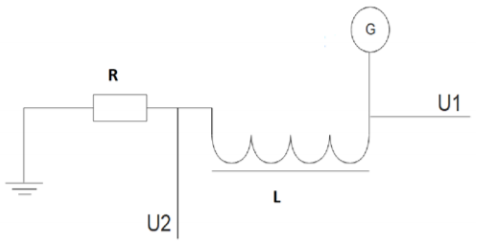
\includegraphics[width=.75\linewidth]{схема.png}
				\caption{Схема измерения индуктивности. $R$ – резистор сопротивлением 95 Ом, $L$ – катушка, индуктивность которой требуется измерить, $G$ – выход встроенного	генератора осциллографа, $U_1$ и $U_2$ – напряжения, измеряемое на первом и втором каналах осциллографа. Земля у генератора и обоих входов осциллографа общая.}
				\label{fig1}
			\end{figure}
			\newpage
			С генератора подается синусоидальный сигнал с амплитудой 12 В. В приближении, что резистор имеет только активное сопротивление, а катушка только реактивное можно рассчитать импеданс катушки $Z_L = i \omega L$ зная $U_1$, $U_2$ и $R$. Полный импеданс всей цепи равен $Z_\Sigma =	R + i \omega L$. Тогда модули (и амплитуды) тока и напряжения в цепи связаны следующим образом: $U_0 = I_0 \sqrt{R^2 + (\omega L)^2}$. Также из этого легко найти модуль тангенса разности фаз между током и напряжением: $tan(\phi) = \frac{\omega L}{R}$. Измеряемое напряжение $U_2$ равно произведению величины тока в цепи на сопротивление $R$, из это получим связь между $U_1$ и $U_2$: $\frac{U_1}{U_2} = \sqrt{1 + (\frac{\omega L}{R})^2}$, из которой можно найти индуктивность $L$. Из этого соотношения легко понять требования на величину сопротивления $R$ и частоту $\omega$: они должны быть такими, чтобы величина $\frac{\omega L}{R}$ заметно превышала единицу, иначе измерения будут неточными.
		\subsection{Ход работы}
			В первую очередь требовалось сделать катушку — намотать медную проволоку на
			ферритовый сердечник. Мы взяли уже намотанную катушку, измерили ее геометрические размеры. Катушка была намотана из толстой медной проволоки и состояла из 42 витков.
			Далее была собрана схема (\ref{fig1}). С помощью осциллографа были измерены напряжения на катушке для токов на различных частотах, затем определены различные значения выражения $\frac{R}{2\pi}\sqrt{(\frac{U_1}{U_2})^2 - 1}$ при различных значениях частоты.
		\subsection{Анализ данных}
			По полученным точкам были построены прямые по МНК и взвешенному МНК, коэффициентом которых является искомая индуктивность катушки.
			\begin{figure}[h]
				\centering
				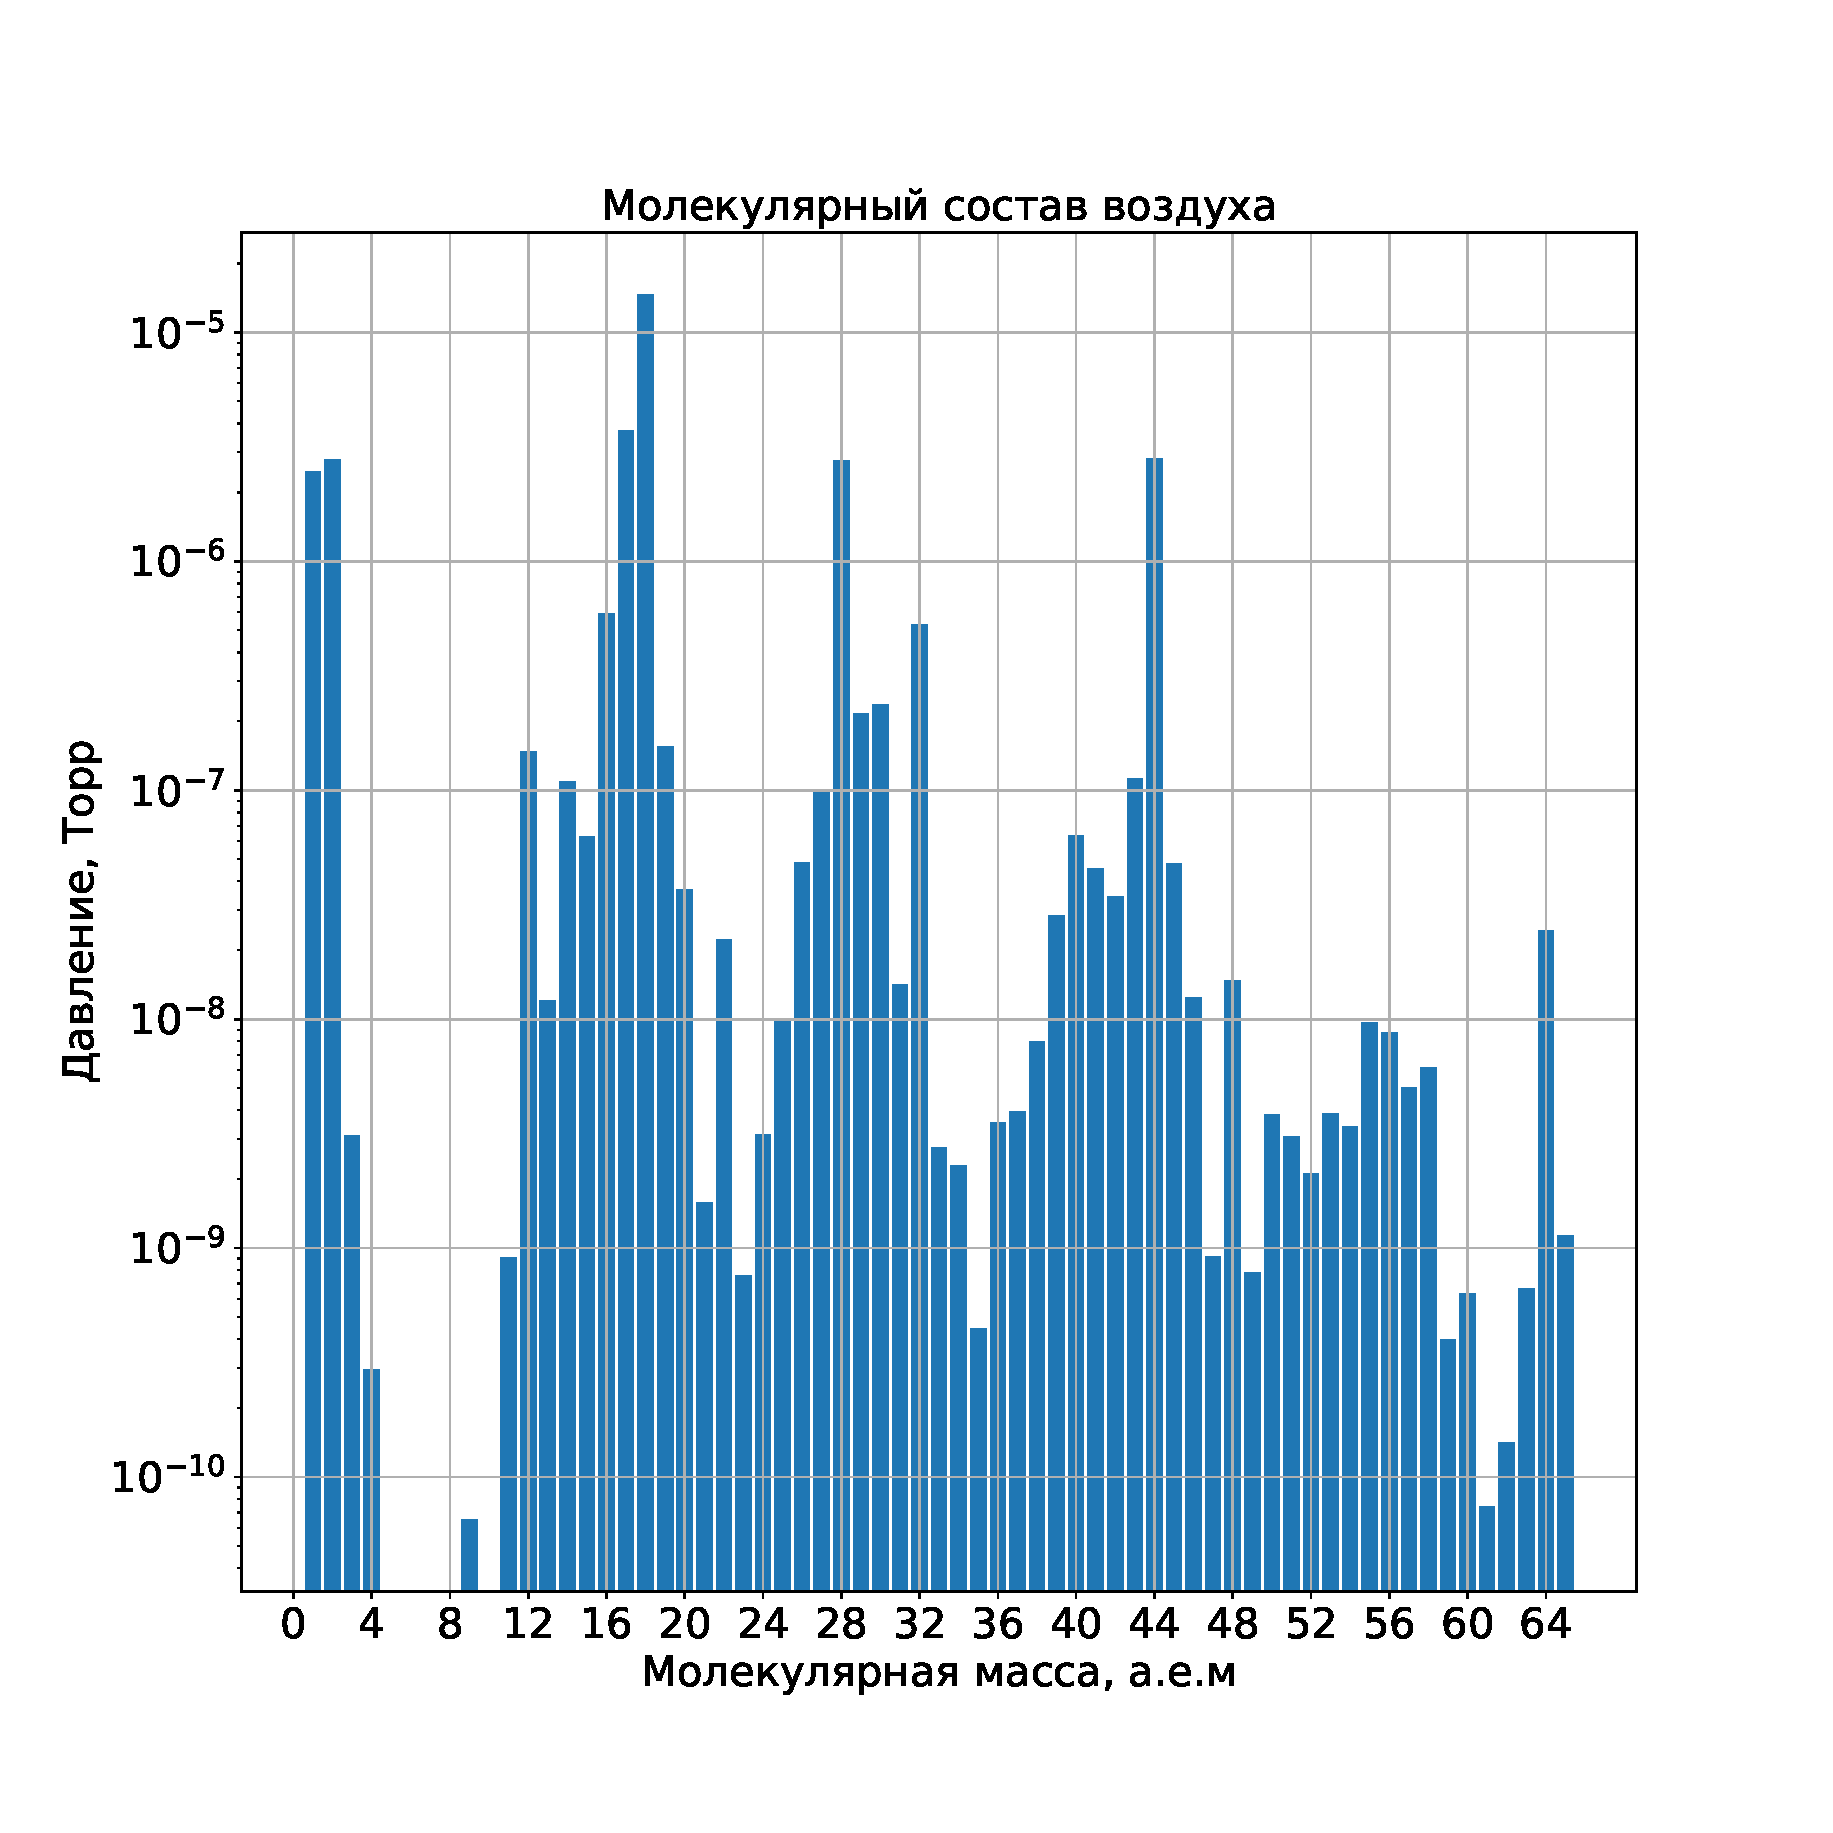
\includegraphics[width=.80\linewidth]{Lab2_1.eps}
				\caption{На графике изображены две прямые: прямая, построенная по экспериментальным данным с помощью МНК и прямая, построенная с помощью взвешенного МНК}
				\label{fig2}
			\end{figure} 
			\newpage
			За основу был взят график, построенный по взвешенному МНК, так как при предыдущих измерениях индуктивности катушки получившийся результат лучше соотносился с заявленной индуктивностью и показателями точных приборов. Получившаяся индуктивность с учетом погрешностей:
			\begin{equation}	
				L = 2.73 \pm 0.10\text{мГн}
			\end{equation}
			С помощью вычисленной индуктивности можно найти магнитную проницаемость:
			\begin{equation}
				\mu = 2.08 \pm 0.08\frac{\text{Гн}}{\text{м}}
			\end{equation}
	\section{Гистерезис}
		\subsection{Теория работы}
			Для получения картины магнитного гистерезиса необходимо собрать одну из следующих схем:
			\begin{figure}[h]
				\centering
				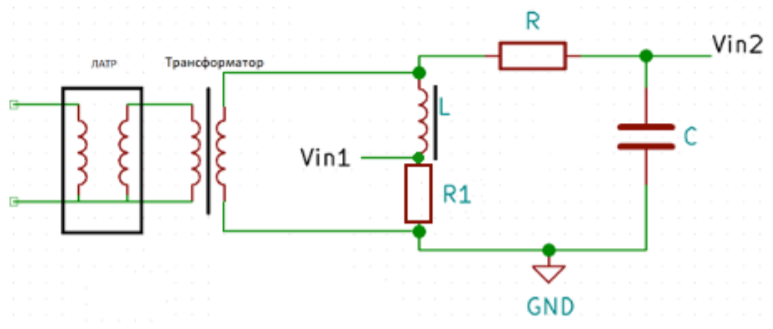
\includegraphics[width=0.9\linewidth]{схема2.png}
				\caption{Схема измерительной цепи с одной катушкой}
				\label{fig3}
			\end{figure}
			\newline
			\begin{figure}[h]
				\centering
				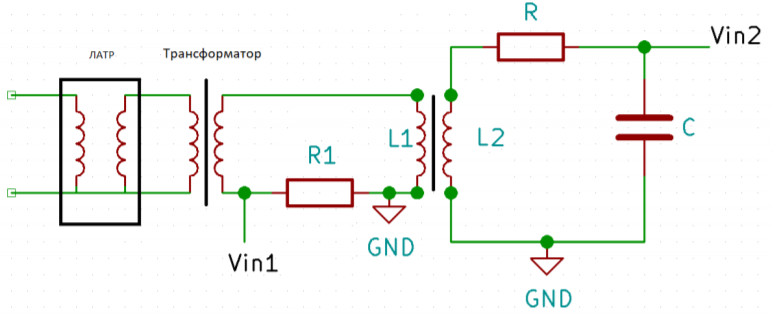
\includegraphics[width=0.9\linewidth]{схема3.png}
				\caption{Схема измерительной цепи с двумя катушками}
				\label{fig3}
			\end{figure}
			\newpage
			Принципиально схемы отличаются мало. В обеих ЛАТР (лабораторный автотрансформатор) используется для питания схемы от сети и регулировки силы тока. Понижающий трансформатор нужен для повышения выходного тока и гальванической развязки схемы от сети. Резистор $R_1$ малого сопротивления ($0.1-1$ Ом) необходим для измерения силы тока, текущего через катушку, $L (L1)$ – собственно катушка из медной проволоки, намотанная на образец. Сопротивление $R$ (номиналом $820$ кОм) и конденсатор $С$ (емкостью в $1$ мкФ) образуют интегрирующую напряжение на катушке цепочку. Напряжение ${\text{Vin}}_1$, пропорциональное току через катушку и, соответственно, напряженности поля $H$ в ней, и напряжение ${\text{Vin}}_2$, пропорциональное интегралу напряжения на катушке и, следовательно потоку и индукции поля B через нее, подаются на два канала осциллографа. 
			Далее, настроив коэффициенты усиления каналов осциллографа и напряжение на входе ЛАТРа можно получить на экране осциллографа изображение петли гистерезиса. Это изображение можно записать (например, на flesh накопитель) и перерисовать в координатах B(H), получив в результате картину магнитного гистерезиса в образце. Cвязь напряженности поля H и тока в цепи I находится по теореме о циркуляции: $\oint\limits\mathbf{H}\cdot d\mathbf{l} = I$, откуда $H = \frac{N_1 I}{\pi D}$, где N1 – число витков в первой катушке, D – средний диаметр тороидального сердечника.
			Связан с напряжением $\text{Vin}_1$ по закону Ома: $\text{Vin}_1 = R_1 I$. Напряжение на катушке (первой или второй) по закону Фарадея пропорционально производной индукции поля B в сердечнике: $V = -\frac{d\Phi}{dt} = -SN_i\frac{dB}{dt}$. Здесь $S$ – площадь поперечного сечения тороидального сердечника, $N_i$ - число витков в катушке. Для того чтобы	измерять сигнал пропорциональный индукции поля используется интегрирующая цепочка из сопротивления $R$ емкости $С$. Можно показать, что если постоянная времени цепочки $RC$ значительно превышает период изменения сигнала (в данном случае это период колебания напряжения в сети электроснабжения равный 17 мс), то напряжение на конденсаторе $\text{Vin}_2$	равно $\frac{1}{RC}\int V dt = \frac{1}{RC}S N_1 B$. Отсюда $B = V_2 R C \frac{1}{S N_2}$ Тогда напряжение $\text{Vin}_2$ пропорционально индукции поля в образце. Намагниченность $\mathbf{M}$ связана с полем соотношением $\mathbf{B} =\mu_0(\mathbf{H} + \textbf{M})$. Магнитная восприимчивость в общем случае равна $\chi = \frac{dM}{dH}$. Индуктивность тороидальной катушки по известной формуле $L = N^2 \cdot \frac{\mu_0 \mu h}{2 \pi} \cdot \ln{\frac{R}{r}}$, где $h$ - ширина сердечника, $R$ - наружный радиус, $r$ - внутренний радиус тора.
		\subsection{Ход работы}
			В ходе работы были собраны обе схемы. Для второй схемы потребовалось намотать на исходную катушку вторую катушку из 56 витков. Провода для нее использовались тонкие, так как по данной катушке текли небольшие токи. Данные снимались с помощью цифрового осциллографа для дальнейшего анализа.
		\subsection{Анализ данных}
			\subsubsection{Первая схема}
				Для первой схемы был получен только один график петли гистерезиса, так как уже на малых напряжениях картина получалась искаженной. 
				\begin{figure}[h!]
					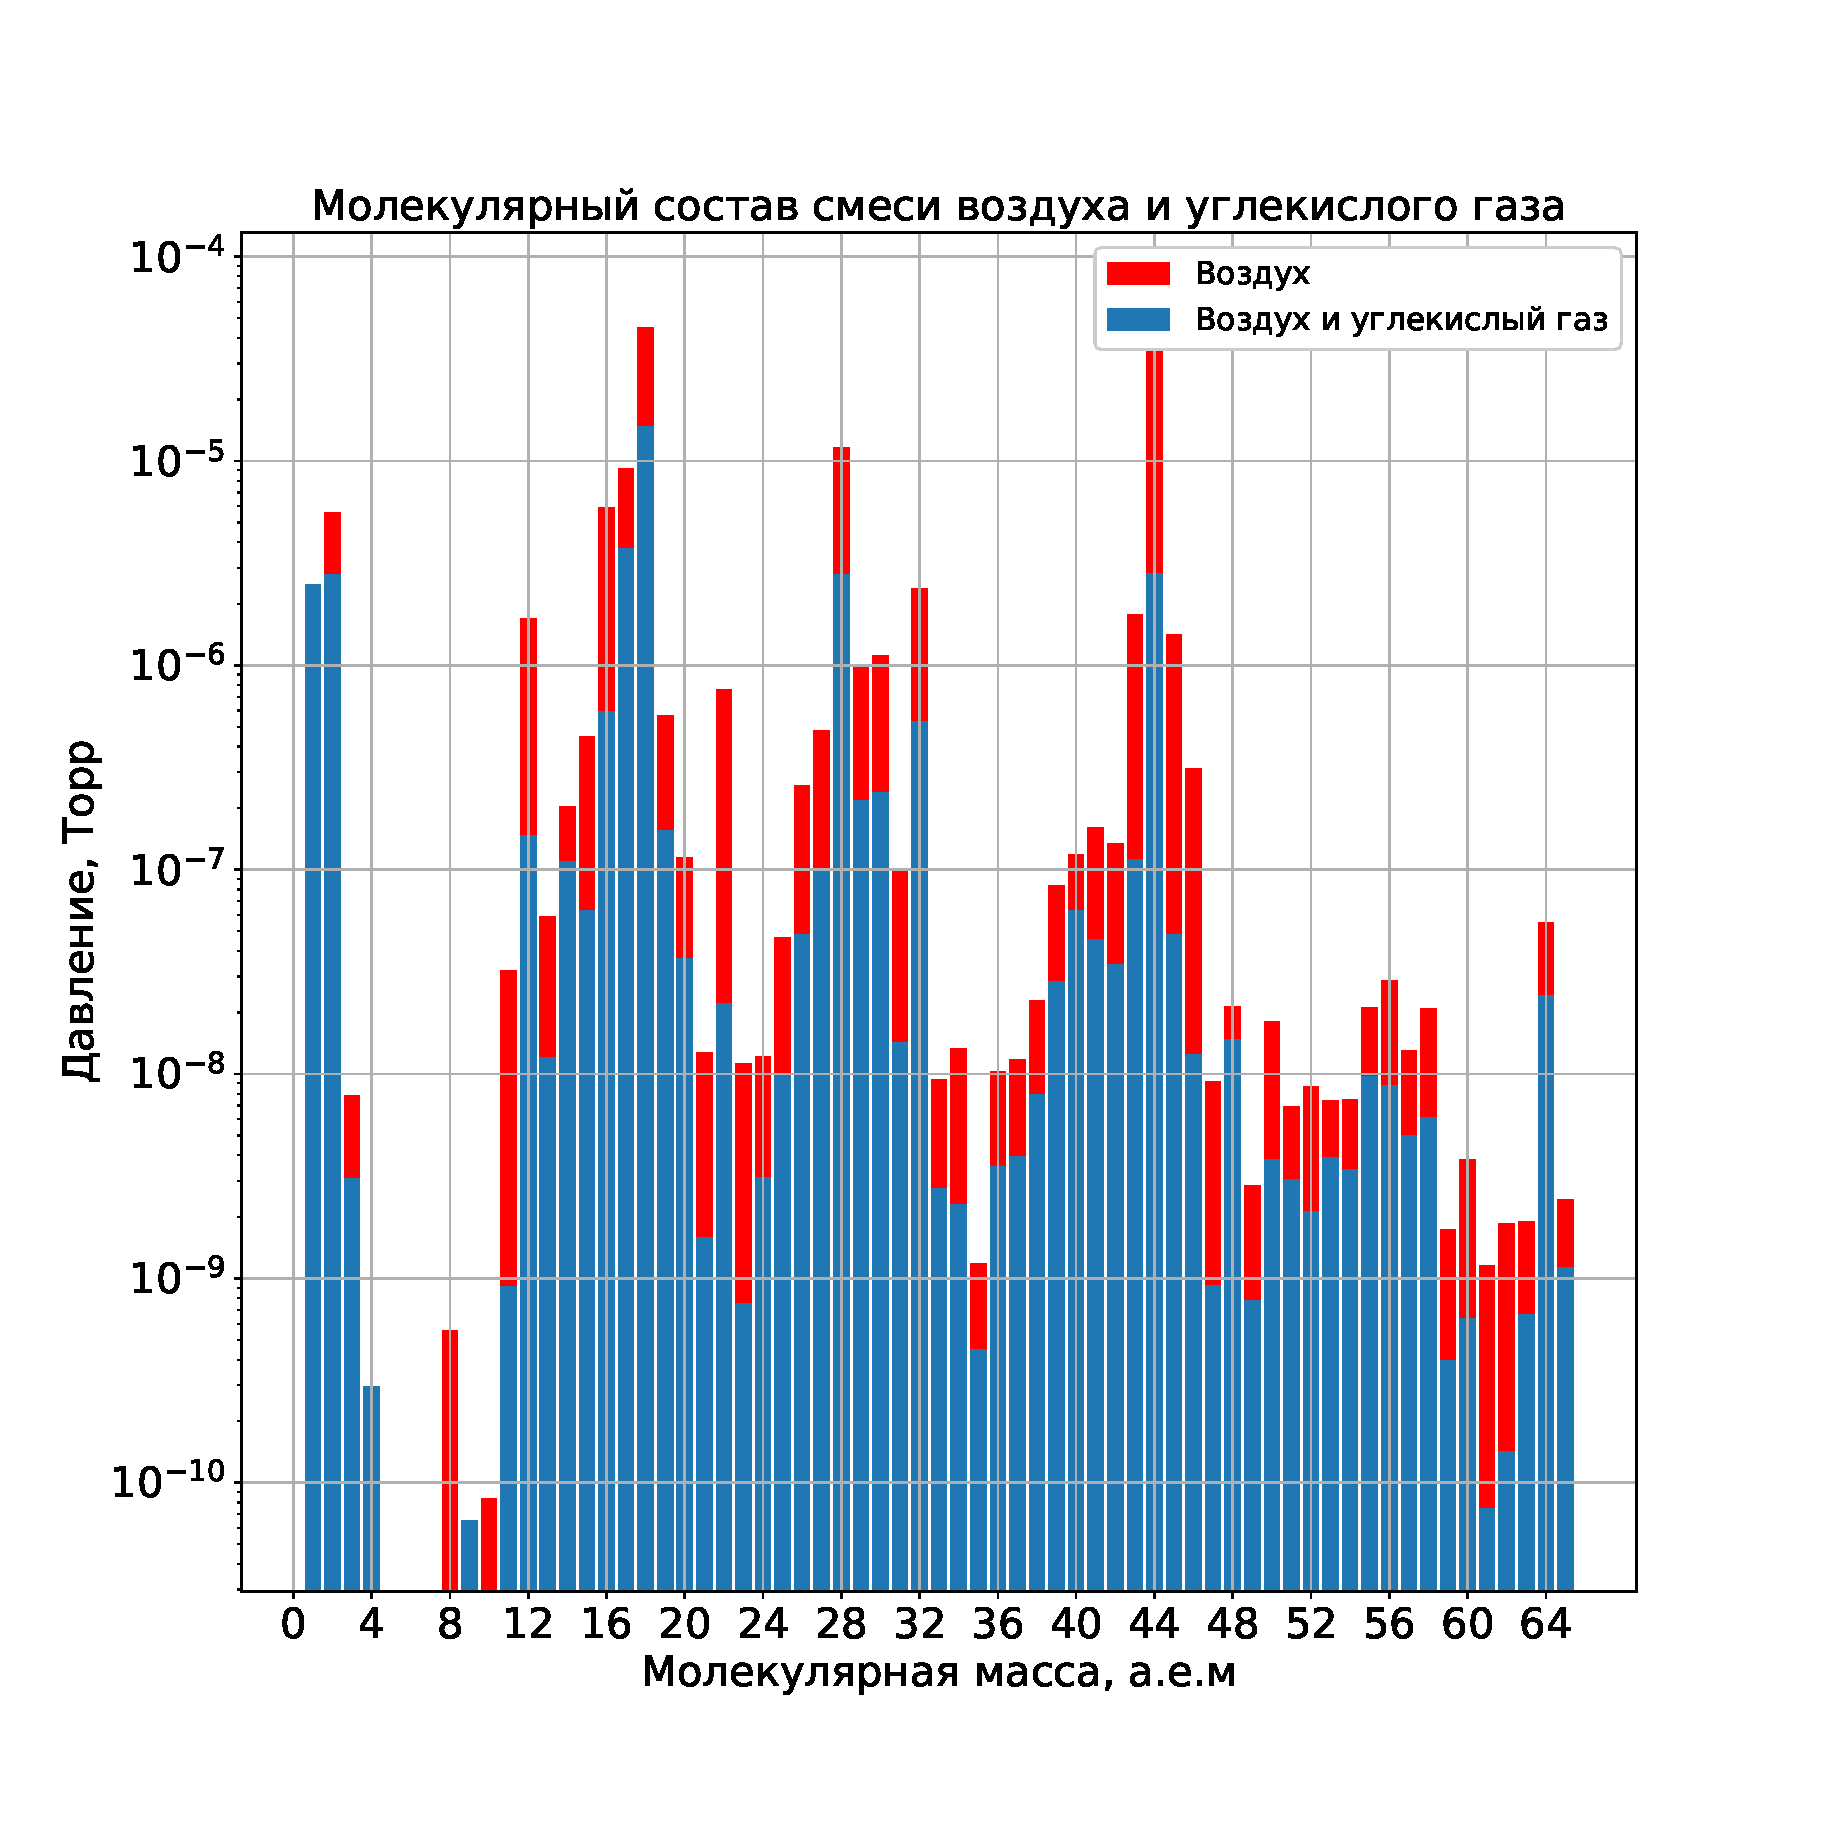
\includegraphics[width=1.0\linewidth]{Lab2_2.eps}
					\caption{Петля гистерезиса для ферритового сердечника. Схема 1}
					\label{fig5}
				\end{figure}
				\newpage
			\subsubsection{Вторая схема}
				Для второй схемы было получено больше неискаженных графиков для разных напряжений на ЛАТР. Поэтому все расчеты было решено проводить именно по данным, полученным со второй схемы.
				\begin{figure}[h!]
					\centering
					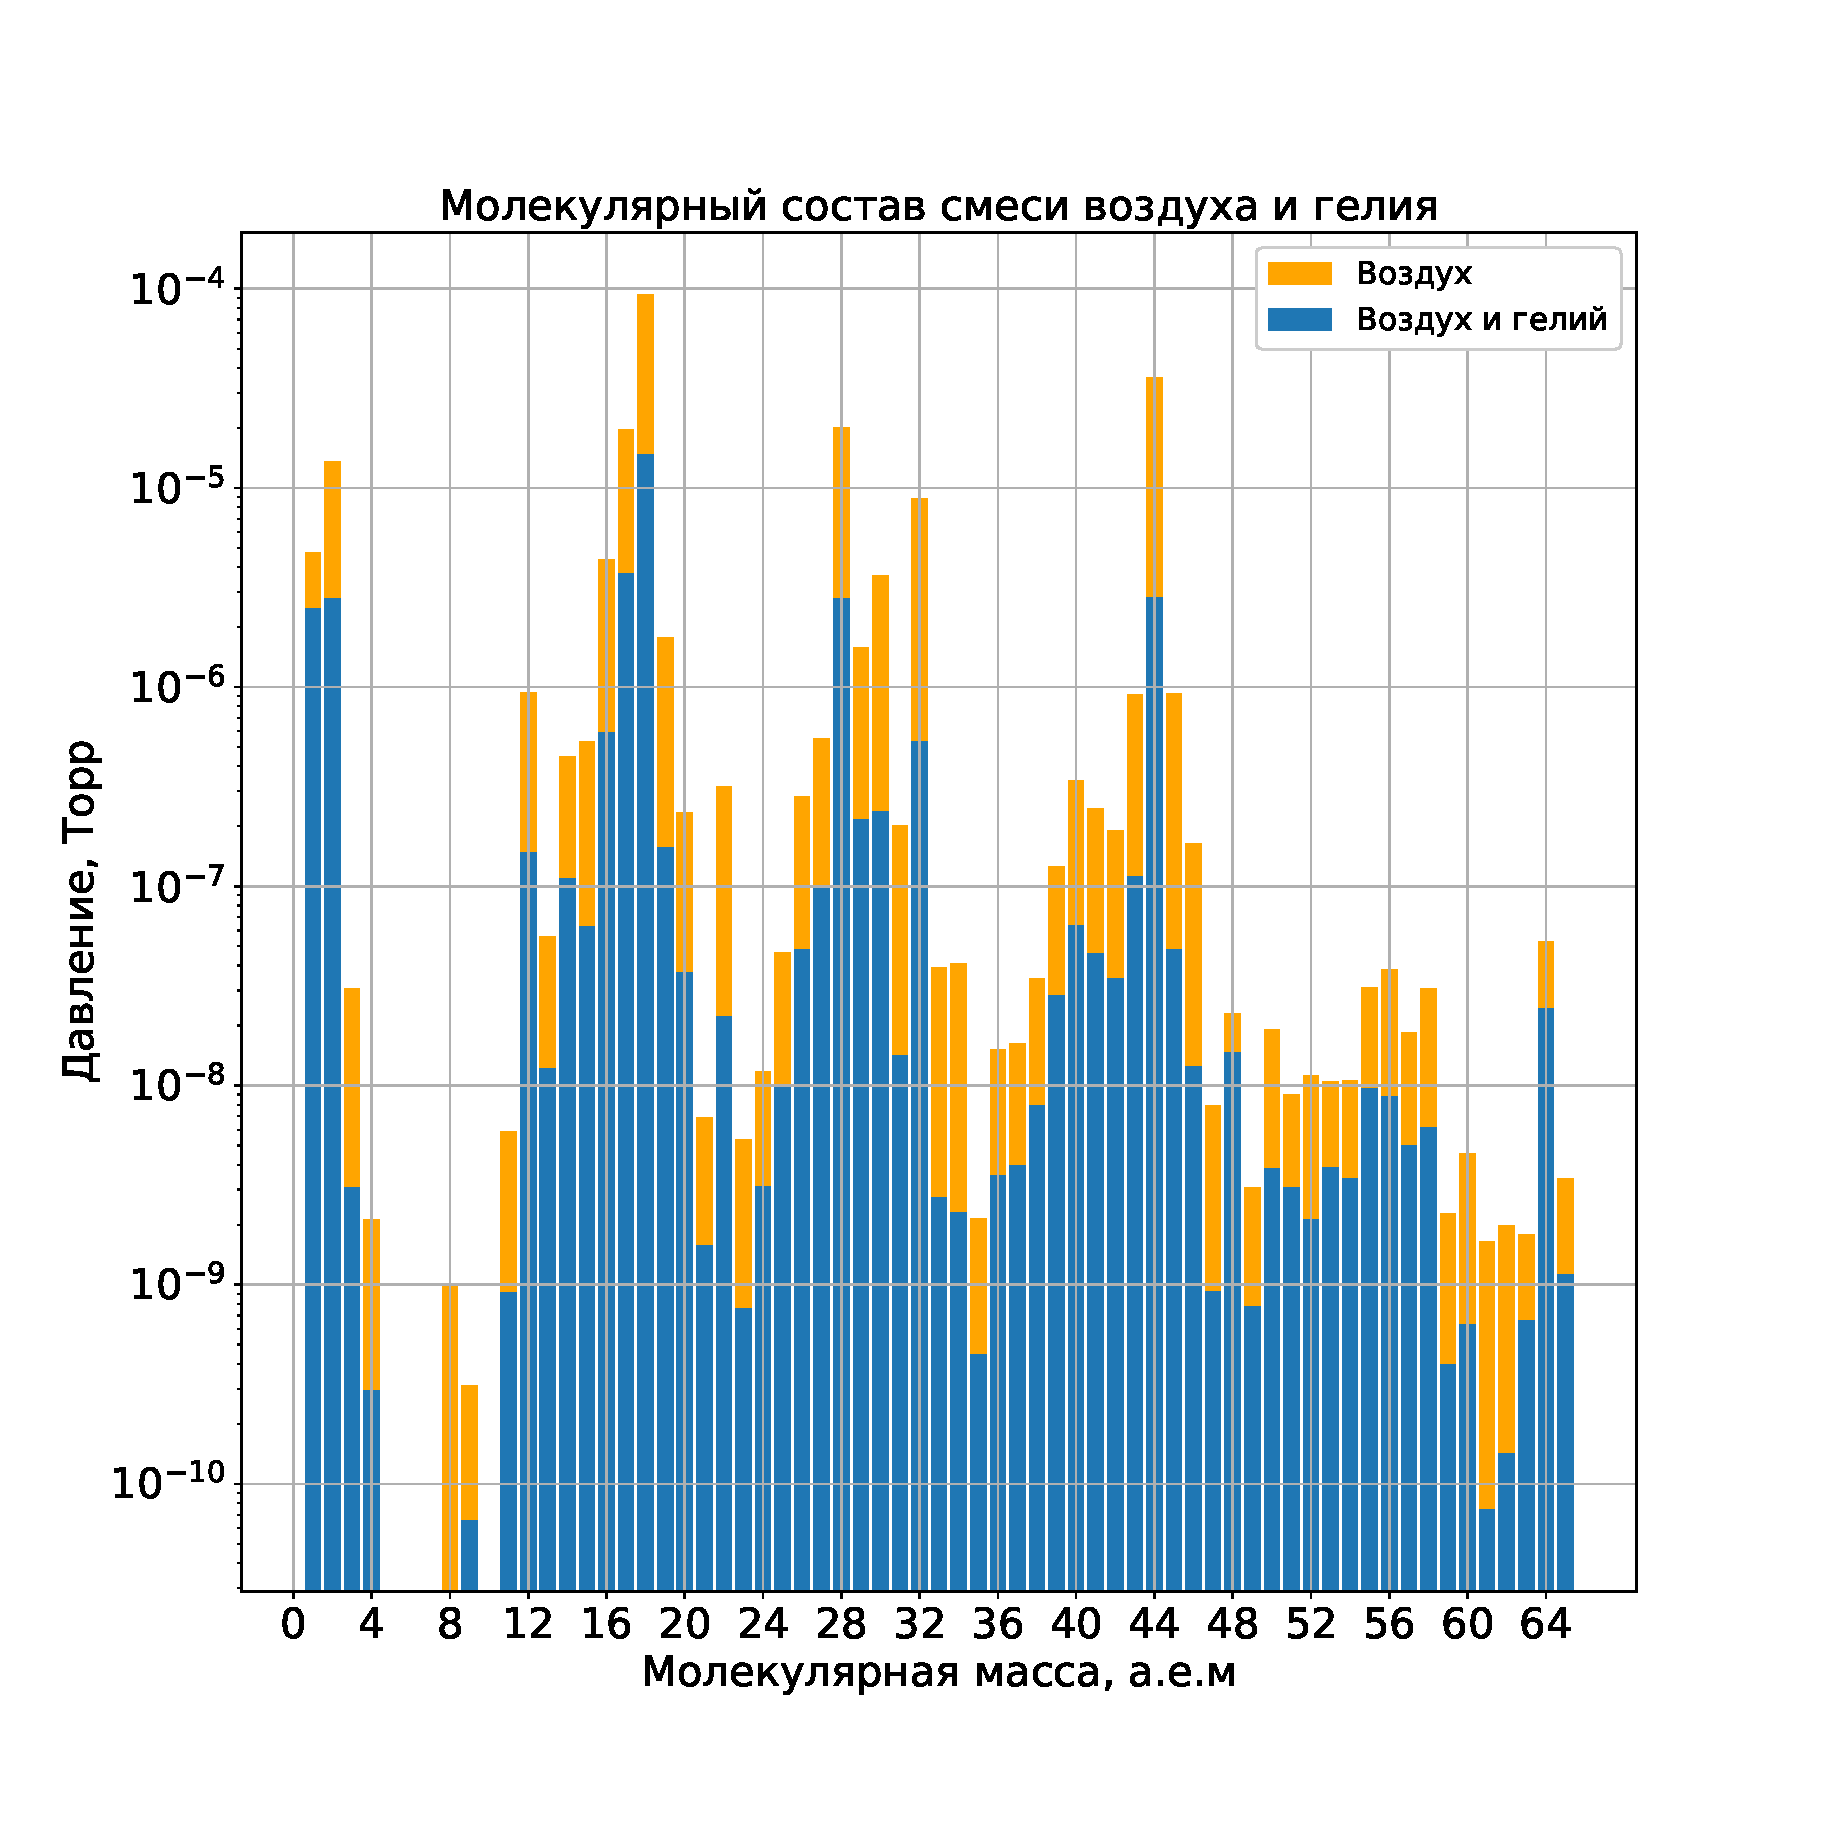
\includegraphics[width=1.0\linewidth]{Lab2_3.eps}
					\caption{Петли гистерезиса при разных максимальных токах в цепи. Схема 2}
					\label{fig6}
				\end{figure}
				\newpage
			\subsubsection{Намагниченность}
				Получив зависимость $B(H)$, перестроим ее в координатах $M(H)$, воспользовавшись соотношением из теории.
				\begin{figure}[h!]
					\centering
					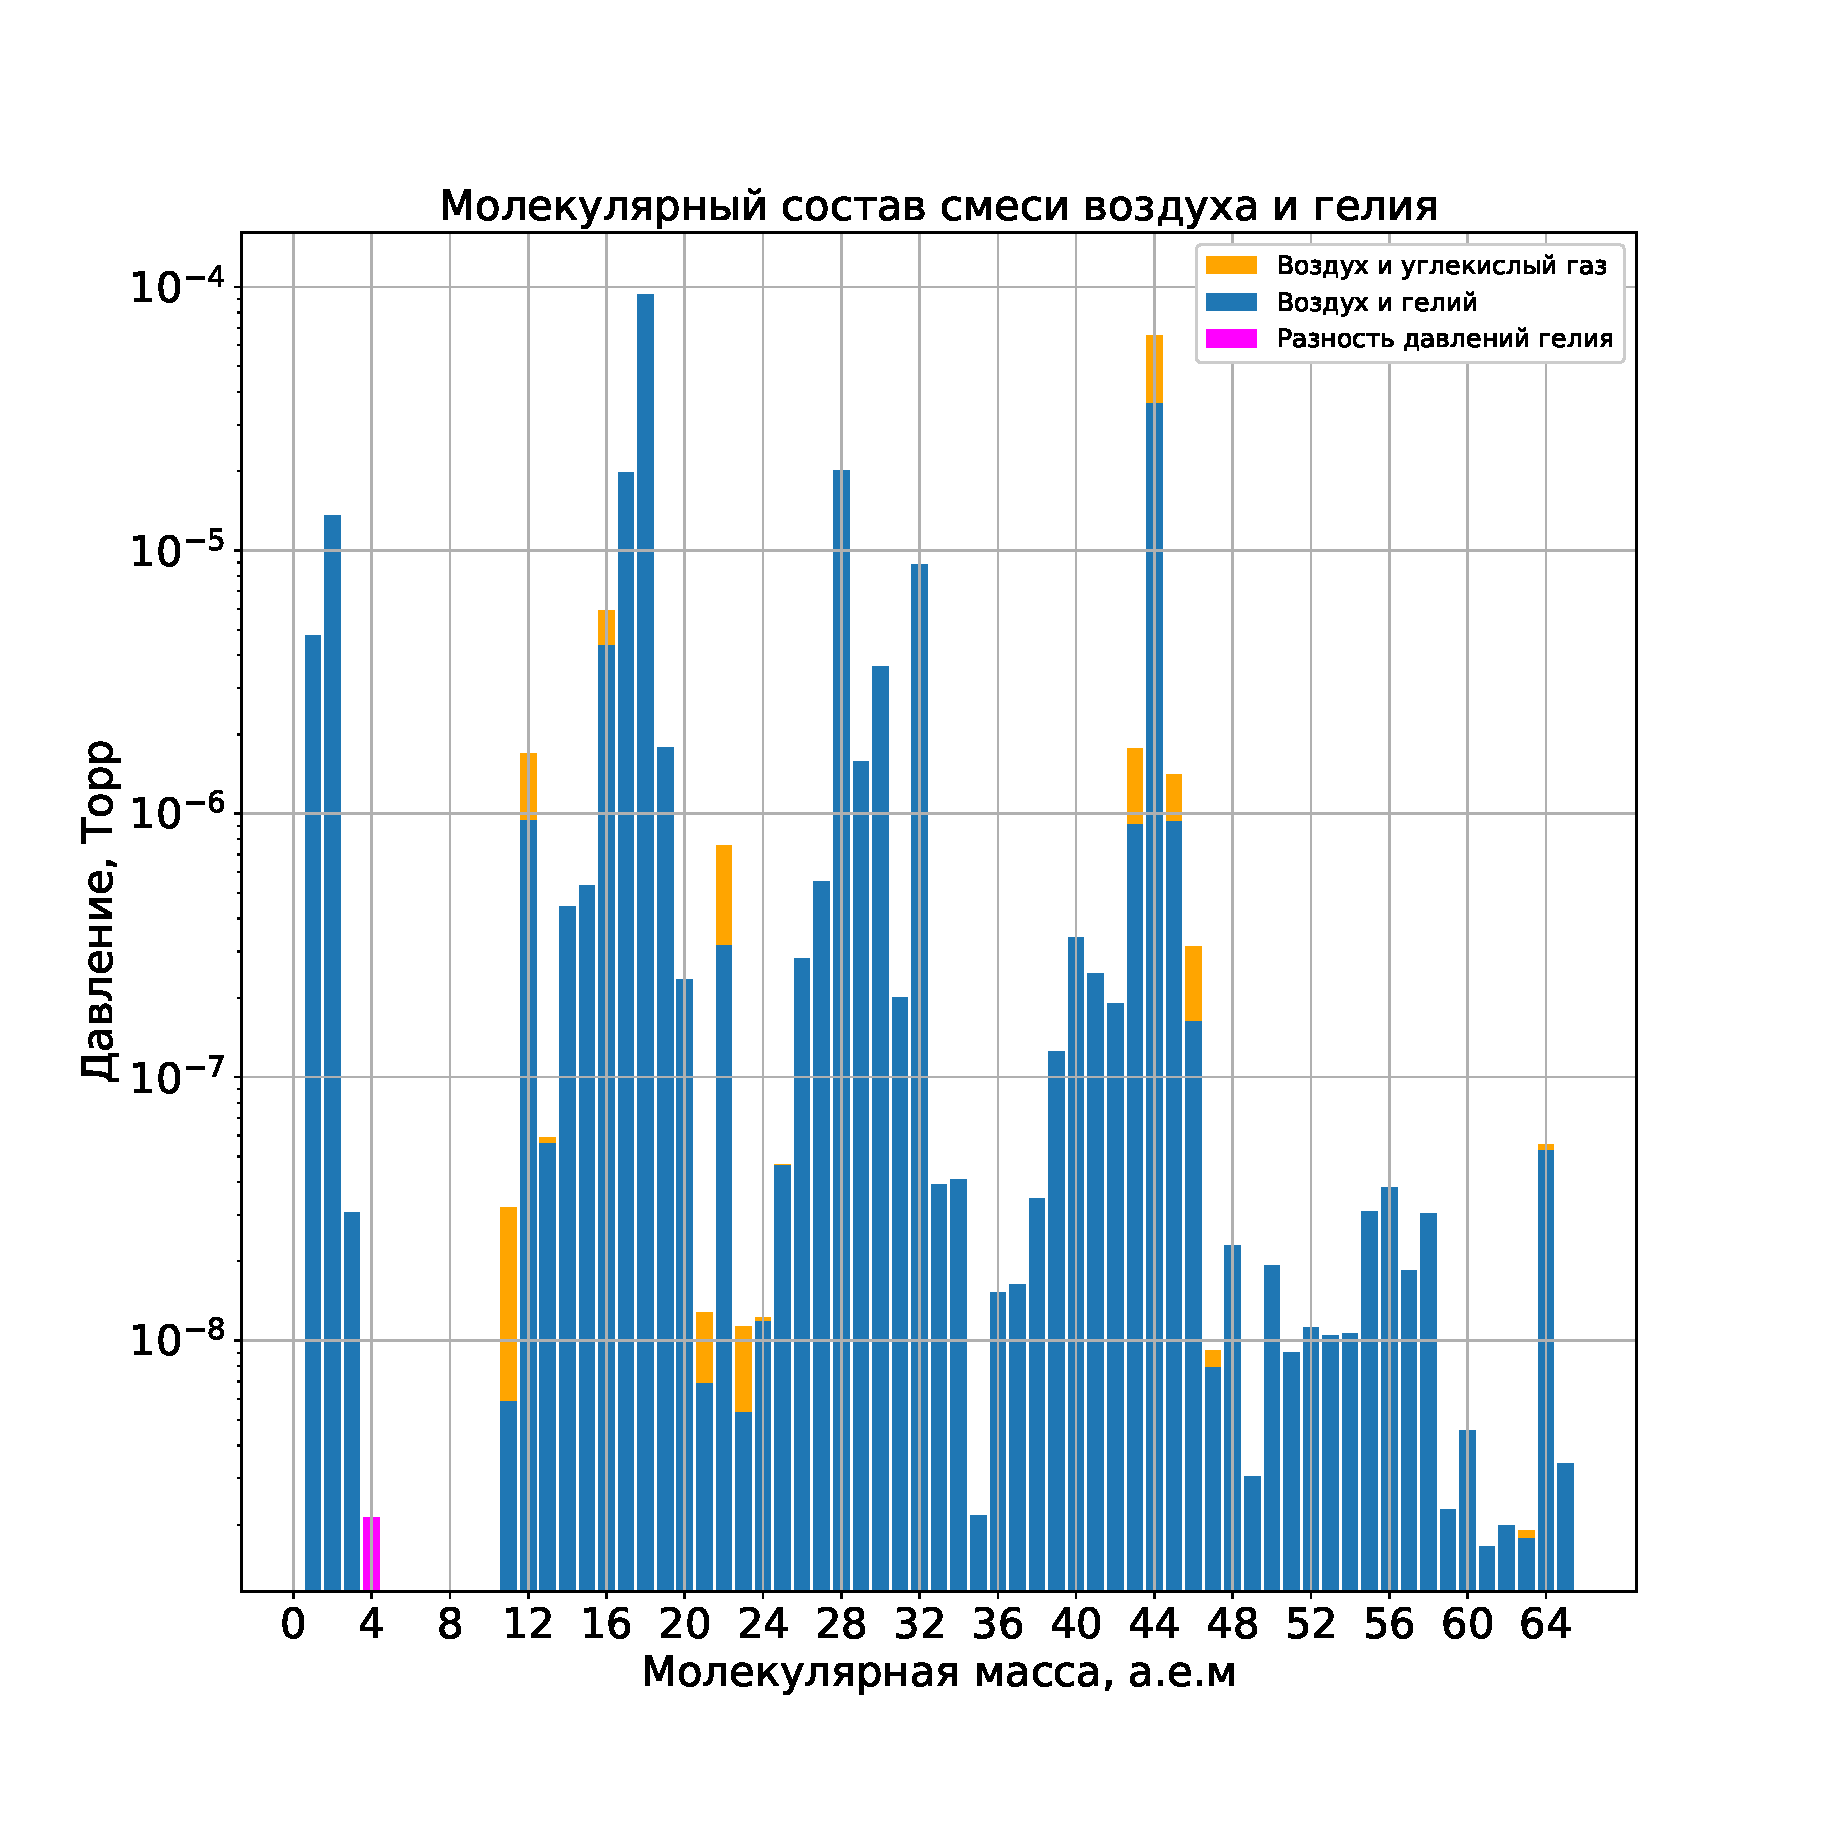
\includegraphics[width=1.0\linewidth]{Lab2_4.eps}
					\caption{Зависимость $M(H)$ при разных максимальных токах в цепи. Схема 2}
					\label{fig7}
				\end{figure}
				\newpage
				Как и следовало ожидать, получился гистерезис.
			\subsubsection{Магнитная восприимчивость}
				В случае гистерезиса, про магнитную восприимчивость корректно говорить как про переменную величину, равную производной $\frac{dM}{dH}$. Построим график зависимости $\chi(H)$
				\begin{figure}[h!]
					\centering
					\includegraphics[width=1.0\linewidth]{Lab2_5.eps}
					\caption{Зависимость магнитной восприимчивости от поля. Схема 2}
					\label{fig8}
				\end{figure}
				\newpage
				Рассматривая положительную часть графика, можно увидеть, что магнитная восприимчивость по увеличению поля увеличивается, затем достигает максимума и убывает к нулю.
			\subsubsection{Коэрцитивная сила и остаточная намагниченность}
				По данным, полученным при разных значениях тока найдем пересечения петли с осями $B$ и $H$, значения $\pm H_c$ и $\pm B_r$ соответственно будут называться коэрцитивной силой и остаточной намагниченностью. Усреднив абсолютные значения $B_r$ и $H_c$ (они разные, так как петля неидеально симметрична) для разных значений максимального тока в цепи получилим разные значения $B_r$ и $H_c$. Значит, про значение этих параметров не очень интересно говорить при фиксированном значении силы тока. Построим по нашим четырем петлям зависимости $H_c(I_{max})$ и $B_r(I_{max})$.
				\begin{figure}[h]
					\centering
					\includegraphics[width=0.8\linewidth]{Lab2_6.eps}
					\caption{Зависимость коэрцитивной силы от максимальной силы тока в цепи. Схема 2}
					\label{fig9}
				\end{figure}
				\newpage
				\begin{figure}[h]
					\centering
					\includegraphics[width=0.8\linewidth]{Lab2_7.eps}
					\caption{Зависимость отстаточной намагниченности от силы тока. Схема 2}
					\label{fig9}
				\end{figure}
				По получившемуся результату можно предположить, что коэрцитивная сила ведет себя линейно по отношению к току(на графике изображена одна дополнительная точка для эксперимента с самым большим током. Если рассматривать только те графики, на которых $H = 0$ вне района насыщения (таких точек только 3), то линейно по отношению к максимальному току ведет себя и остаточная намагниченность.
				\newline
				\begin{equation}
					\begin{gathered}
				 		\text{При } I = 5.77 \text{А}:
						\begin{gathered}
							H_c\approx 2.68 \; \frac{\text{А}}{\text{мм}}\\
							B_r\approx 4.05 \; \text{Тл}
						\end{gathered}\\ \\
							\text{При } I = 14.38 \text{А}:
						\begin{gathered}
							H_c\approx 4.99 \; \frac{\text{А}}{\text{мм}}\\
							B_r\approx 4.91 \; \text{Тл}
						\end{gathered}\\ \\
					\end{gathered}
				\end{equation}
				\begin{equation}
					\begin{gathered}
							\text{При } I = 19.87 \text{А}:
						\begin{gathered}
							H_c\approx 6.51 \; \frac{\text{А}}{\text{мм}}\\
							B_r\approx 5.11 \; \text{Тл}
						\end{gathered}\\ \\
							\text{При } I = 37.36 \text{А}:
						\begin{gathered}
							H_c\approx 12.07 \; \frac{\text{А}}{\text{мм}}\\
							B_r\approx 5.41 \; \text{ Тл}
						\end{gathered}\\ \\
							\text{При } I = 60.20 \text{А}:
						\begin{gathered}
							H_c\approx 19.54 \; \frac{\text{А}}{\text{мм}}\\
							B_r\approx 3.32 \; \text{Тл}
						\end{gathered}\\ \\
					\end{gathered}
				\end{equation}
\end{document}